\section{Hårdvarulayout}
    Vi har valt att använda produkter från Fortinet då det finns ett partnersamarbete mellan dem och Netsecure. Vad vi kan se är Fortinets utbud väl tillräckligt för den utrustning vi har valt och priset har legat jämnt eller lägre gentemot andra märken för den prestanda som behövts.

\subsection{Minimikrav}
    \begin{itemize}[noitemsep]
        \item Högst 24 personer på varje site.
        \item Högst 6 kontorsenheter t.ex. printers, ip-telefoner.
        \item Högst 2 AP:s på varje site, dessa ska stödja dual-radio (dvs 2.4 Ghz \& 5Ghz)
        \item Varje site har upp till två anslutningar till core siterna.
        \begin{itemize}[noitemsep]
        	\item En krypterad anslutning över internet med hastighet upp till 100 Mbit/s.
            \item En VPN-anslutning över ett privat nätverk som är isolerat från internet med hastighet upp till 50 Mbit/s.
        \end{itemize}
    \end{itemize}
    
    \noindent Efter dessa minimikrav designades följande topologi för siterna, vilket kan ses i Figur \ref{fig:site-topology}:
    \begin{itemize}[noitemsep]
    	\item En FortiGate 60E-PoE router kopplad till ISP och/eller VPN beroende på det lokala förutsättningarna.
        \item En FortiSwitch 124E kopplad till routern för användare.
        \item Två FortiAP 221C access-punkter kopplade direkt till routern med PoE.
    \end{itemize}
    
 	\begin{figure}[htb]
        \centering
        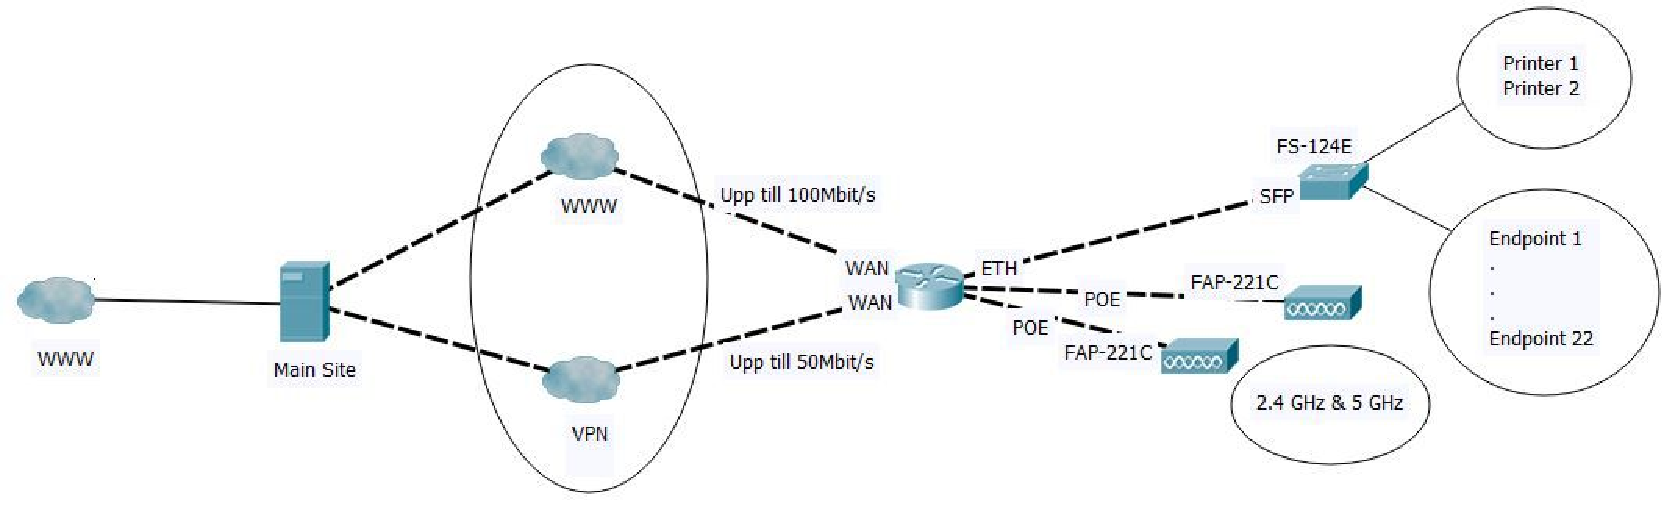
\includegraphics[width=\textwidth]{pics/Topologi_H_rdvara.pdf}
        \caption{Topologi för hårdvarulayout.}
        \label{fig:site-topology}
    \end{figure}

\subsection{Routing \& Brandvägg}
    Routern och brandväggen som valts till projektets lösning är FortiGate 60E-PoE, se Figur \ref{fig:router-60e}. Denna routern valdes för att det är den billigaste router som uppfyller minimikraven på överföringshastigheten även när alla brandväggsfunktioner används. Den har tillräckligt många portar för att täcka de behov som behövs samt PoE som behövs till accesspunkter.
    
    \begin{figure}[htb]
        \centering
        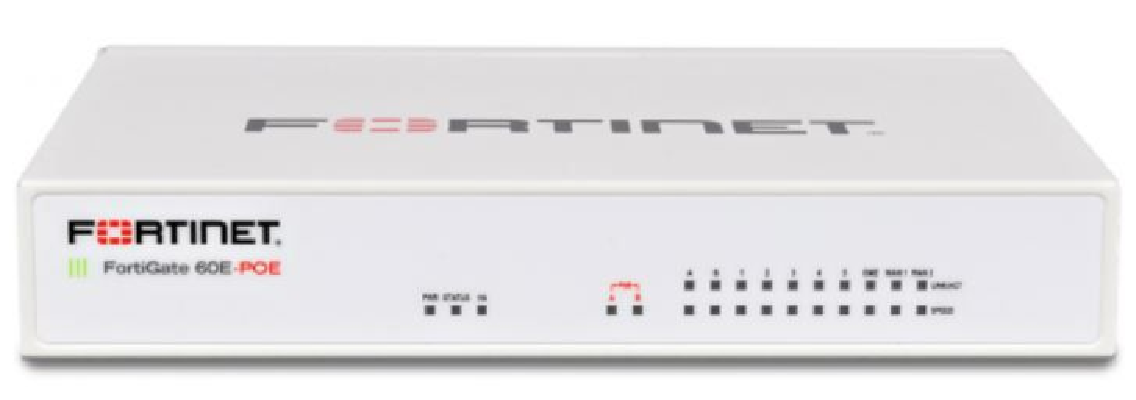
\includegraphics[width=0.95\textwidth, clip, trim={0 0 0 0}]{pics/FortiGate-60E-POE-Frontside.pdf}
        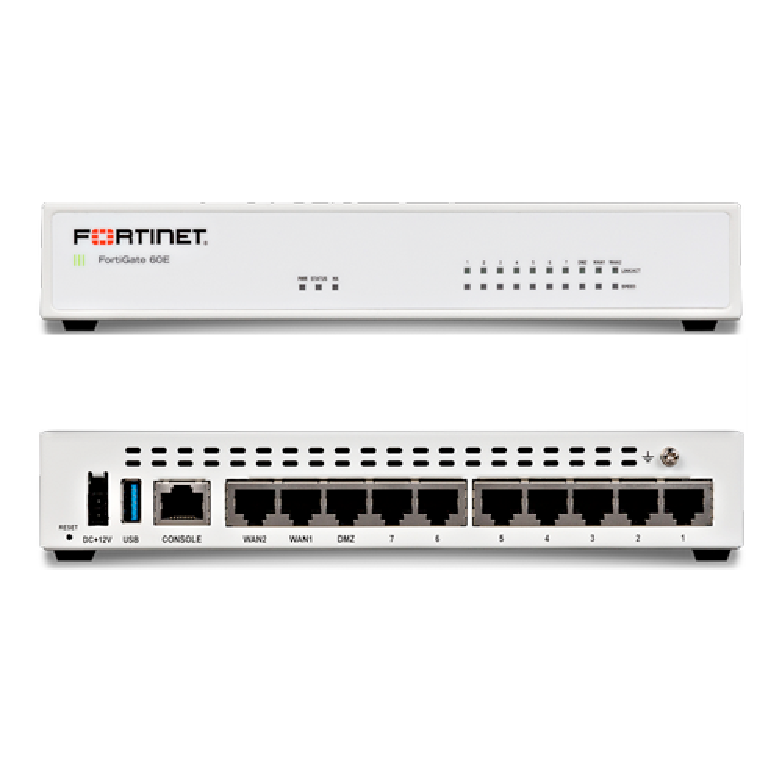
\includegraphics[width=\textwidth, clip, trim={0 3cm 0 6.5cm}]{pics/fortigate-60e-facerear.pdf}
        \caption[FortiGate-60E]{FortiGate 60E-PoE.}
        \label{fig:router-60e}
    \end{figure}

\subsection{Switching}
    FortiSwitch 124E är switchen som valdes och precis som med routern var det priset kontra prestanda som avgjorde valet. FortiSwitch 124E är Fortinets billigaste 24-portars switch och en sådan täcker de maximala antalet användare som kan komma att finnas på vardera site. Switchen kan ses i Figur \ref{fig:switch-124e}.
    
    \begin{figure}[htb]
        \centering
        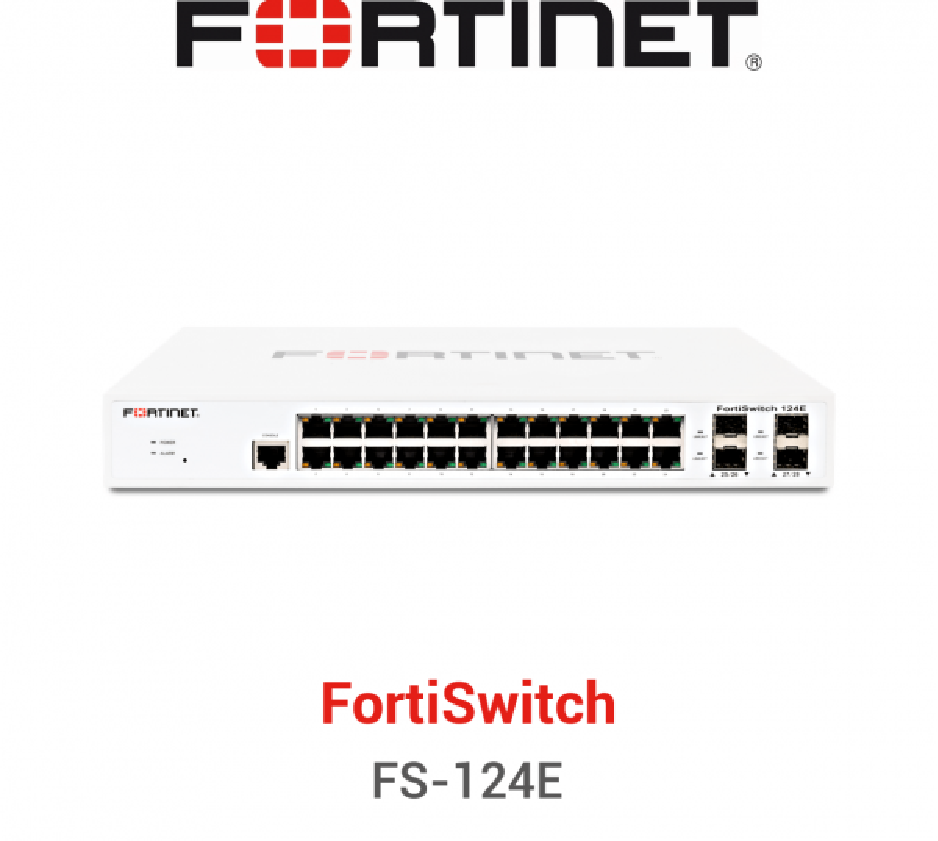
\includegraphics[width=\textwidth,trim={0 5cm 0 5cm}, clip]{pics/FortiSwitch-124E_icon_600x600.pdf}
        \caption{FortiSwitch 124E}
        \label{fig:switch-124e}
    \end{figure}

\newpage
\subsection{Wireless}
    FortiAccessPoint 221C är en av Fortinets enklare trådlösa accesspunkter men innehar tillräckligt med funktionalitet för att täcka de krav som kunden har ställt, exempelvis 2x2 MIMO och dual-radio för att kunna köra både på 2.4Ghz och 5Ghz bandet \cite{FN_FortiAP}. Access-punkten kan ses i Figur \ref{fig:ap-221c}.
    
     \begin{figure}[htb]
        \centering
        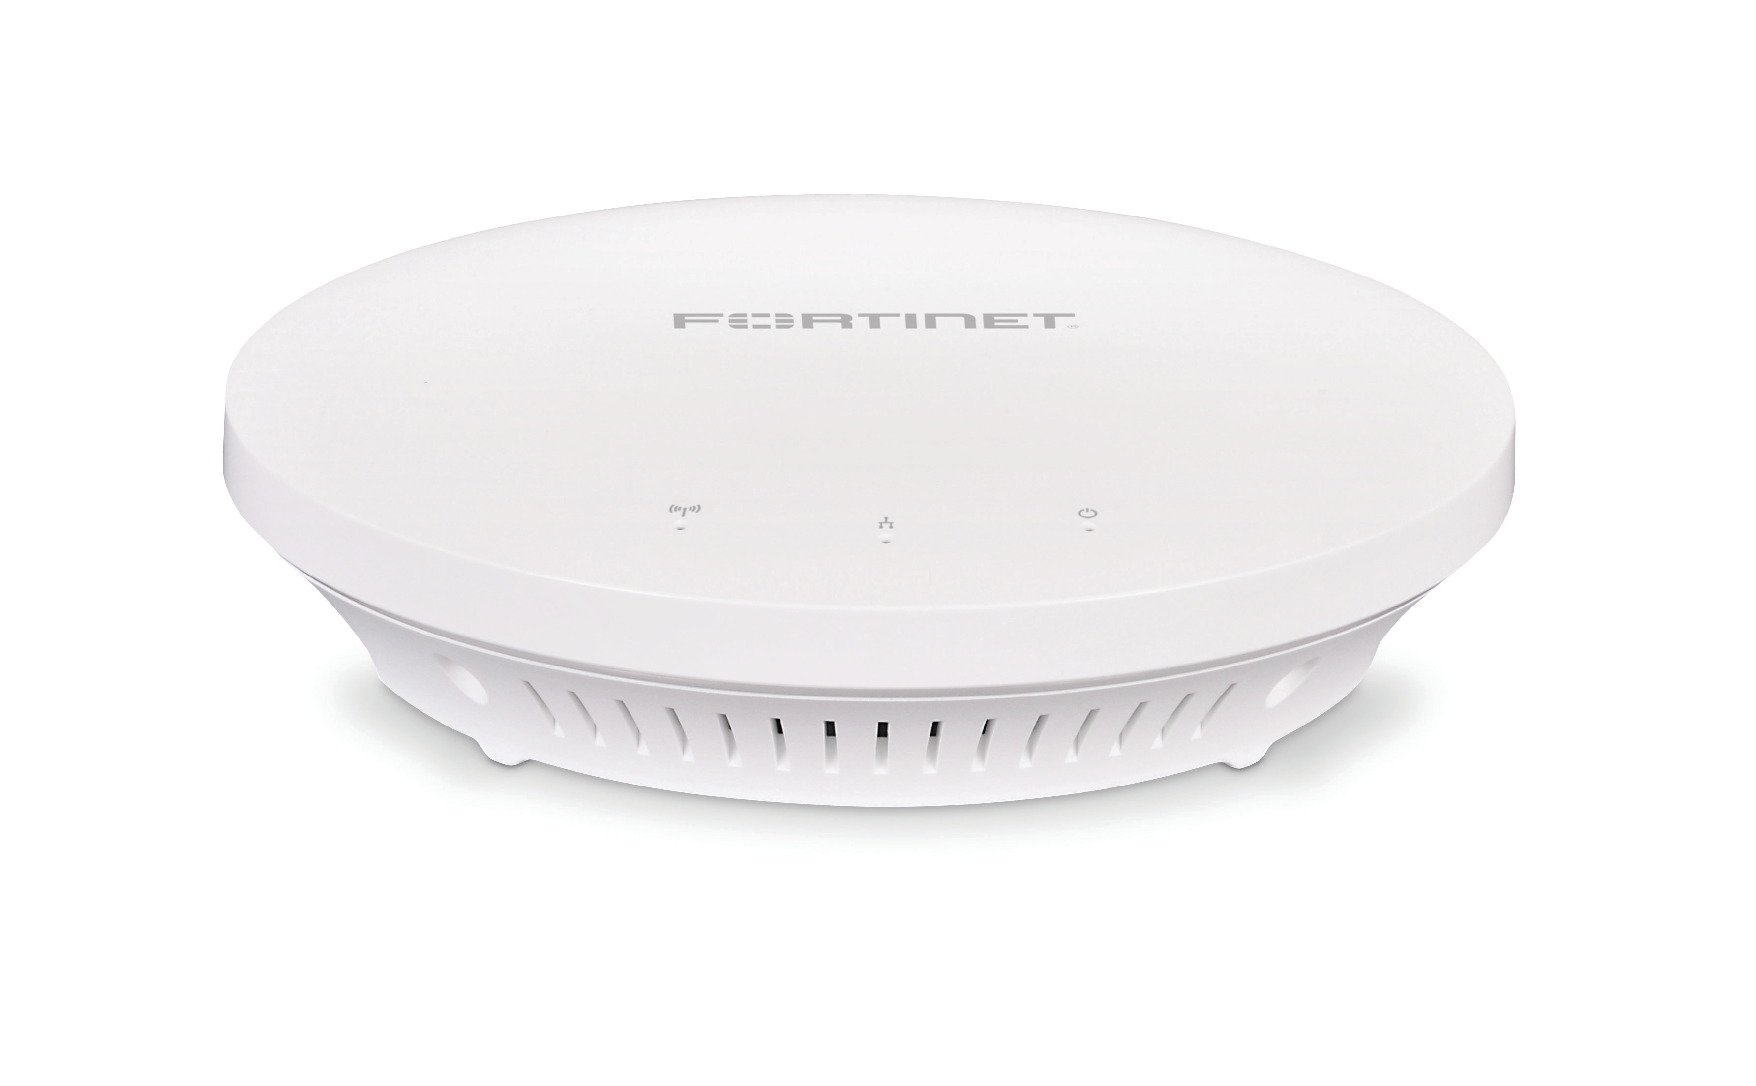
\includegraphics[width=0.8\textwidth,trim={0 3cm 0 1cm}, clip]{pics/FortiAccesspoint-221C.pdf}
        \caption{FortiAccessPoint 221C}
        \label{fig:ap-221c}
    \end{figure}

\subsection{Fysisk Säkerhet}
Vi ger följande rekommendationer för att säkra siternas hårdvara:
    \begin{itemize}[noitemsep]
        \item Låsta rackskåp/dörrar där hårdvara är placerad.
        \item Ge endast fysisk access till personal som anses vara behöriga.
        \item Utbilda personalen på plats.
        \item RJ45-lås på anslutna kablar.
    \end{itemize}




